\parindent 0in
\parskip 0.1in

{\bf Title:  Reduced Order Modeling of heat and fluid flow: Multi-scale
modeling of advanced reactors to enable faster deployment }

{\bf Technical work scope identification: M\&S 1 }

{\bf PI:}
Paul Fischer \\
Department of Computer Science \\
Department of Mechanical Science \& Engineering \\
University of Illinois, Urbana-Champaign \\

{\bf co-PIs:}
Elia Merzari, Pennsylvania State University, \\
Dillon Shaver, Argonne National Laboratory \\

\section{Project Summary}

% \begin{itemize}
% \item
% A summary of the proposed project, including a description of the project and a
% {\em clear explanation of its importance and relevance to the objectives in Part I
% Section A.}
% \item
% Major deliverables and outcomes the R\&D will produce.
% \item
% Timeframe of execution: October 1, 2023--September 30, 2026
% \end{itemize}

\begin{figure}[b!] \centering
    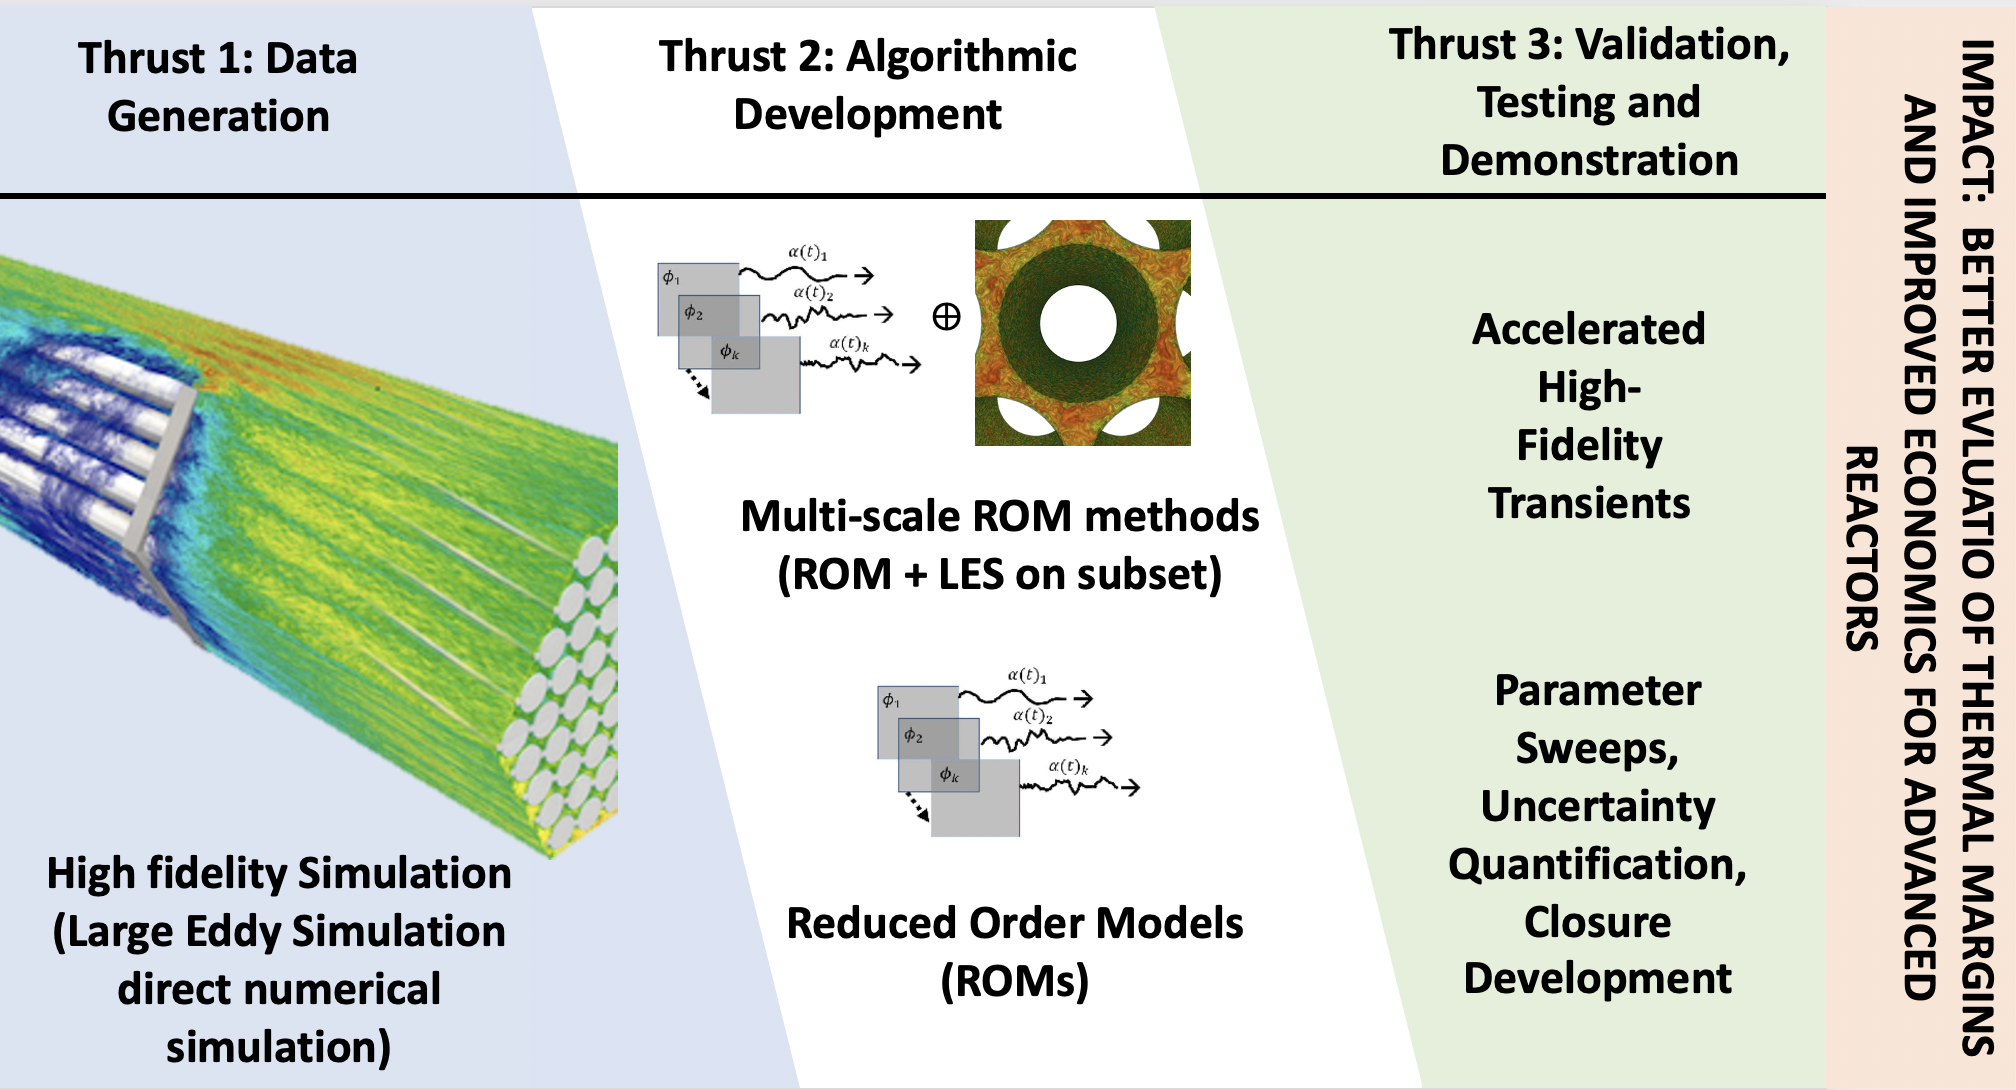
\includegraphics[width = 0.85\textwidth]{figs/fig1.png}
    \caption{Overview of Project with three thrusts: Data generation,
             algorithmic development and validation/demonstration.  \label{fig:sum}}
\end{figure}

We seek \textbf{to develop novel multi-scale algorithmic approaches for the
simulation of heat and fluid flow in advanced reactors}. The methods, which
leverage recent advances in hardware and reduced order modeling approaches,
will enable fast-running simulations of vastly accelerated speed, while
maintaining accuracy comparable to high-fidelity methods such Large Eddy
Simulation (LES) and Direct Numerical Simulation (DNS). These methods will
allow to perform
parameter sweeps to assess uncertainty and develop closures. They will also
enable, for the first time, to perform high fidelity simulation of transients.

Several  advanced reactors concepts are currently being pursued in the United
States, with dozens of companies proposing unique designs. Crucial for their
deployment is the analysis of  reactor transients (e.g., a protected loss of
flow): an essential part of the evaluation of thermal margins and the overall
safety case.  In most cases, licensing will be pursued with established
methods, based on lumped parameter system codes (e.g., SAM \cite{hu2021}).
However, these codes require adequate closures that are typically obtained
empirically and require extensive validation. Furthermore, these methods are
characterized by high level of uncertainty when dealing with complex
three-dimensional turbulent flow, especially in the presence of large
enclosures, mixed convection, and thermal stratification. High-fidelity
simulation on the other hand remains prohibitively expensive, especially for
large parameter sweeps or for the simulation of nuclear transients, and data
remains sparse.

Moreover, as the advanced reactor industry matures and moves past demonstration
projects, economics will become a larger and larger driver. This pressure will
likely push vendors to seek to maximize the economic potential (e.g., higher
power output, higher temperature for process heat, reduced capital cost),
especially as new materials and fuels are introduced. These goals will benefit
from radically improved methods to assess thermal margins that push toward high
fidelity. \textbf{This proposal seeks to develop radically novel algorithmic
approaches to the simulation of advanced reactors, with an unprecedented level
of fidelity, enabling transformative design approaches and improved economics.}
In particular we aim to: 
\begin{enumerate}
%
   \item \textit{Enable the simulation of large parameter sweeps using reduced
   order models developed over a subset of the parameter space.} This approach
   will allow to assess uncertainty of system-level approaches and to develop
   closures.
%
   \item \textit{Enable the accelerated simulation of transients.}
   This approach will allow to assess lower resolution approaches in conjunction
   with experimental data for the simulation of transient.  
\end{enumerate}
As a demonstration application we choose the simulation of Sodium Fast Reactor
(SFR) fuel assemblies under steady-state and transient conditions. \textit{We
emphasize that the methods developed will apply to a broad range of advanced
reactor applications.}

\section{Project Motivation and Technical Objectives}

We propose to leverage ongoing hardware, software, and algorithmic developments
to dramatically enhance thermal-hydraulic analysis capabilities.  The work will
entail combining advanced simulations on DOE's exascale computing platforms
with modern data analysis methods that effectively compress these
first-principle data to efficient exploratory tools based on reduced-order
models (ROMs).
We illustrate the project overview in Fig. \ref{fig:sum}.

\noindent
{\bf High-Fidelity Simulations on DOE Leadership Computers.}
The Department of Energy is in the process of standing up three exascale
computing platforms: Frontier at ORNL, El Capitan at LLNL, and Aurora at ANL.
We have recently demonstrated that it is possible to simulate a single flow
through time for the thermal-hydraulics of a full pebble-bed reactor core
(352,000 pebbles) in just six hours of wall-clock time on the {\em
pre}-exascale machine, Summit, at ORNL \cite{sc22}.   This is an impressive
acheivement as it involves a quarter-trillion degrees-of-freedom, executing a
0.3 seconds per step.  This problem is relatively small by exascale standards,
so it will be possible to explore multiple configurations in this space within
a single annual allocation, which will make it possible to consider parameter
exploration that is critical for analysis and design.

The software that enables this achievement is {\em NekRS}, which is the
GPU-oriented version of the high-order spectral element code, Nek5000, that
is being developed under DOE's Center for Efficient Exascale Discretizations
(CEED). NekRS sustains $\approx$ 0.5--1.0 TFLOPS ($10^{12}$ floating point
operations per second) per MPI rank on current pre-exascale platforms Summit
and Crusher at ORNL and Polaris at ANL.  It is a highly efficient code that
realizes 2--4 TFLOPS/rank on key kernels and 80\% parallel efficiency with
about 2M grid points per rank.  Consequently, a 50B grid-point problem such as
the full pebble-bed reactor core of Fig. \ref{fig:pbr} can effectively use
$P$=25,000 GPUs (or GCDs in the case of Frontier or tiles in the case of
Aurora).  While such a calculation effectively uses all of Summit, it would
fill only a fraction of Frontier or Aurora.  On these platforms, we can
anticipate running larger problems or running at multiple points in the reactor
design space.  Execution times on these platforms can be anticipated to remain
at $\approx$ 0.1--0.3 seconds per step, even with larger problems
running on the full systems.


{\bf Show some scaling plots (Crusher, etc.)}

%% (WHY ROM)
\noindent
{\bf Data-Driven Reduced-Order Models.}
While it is clear that NekRS will be capable of delivering fast turn-around
for reactor-scale simulations on DOE's exascale platforms, the use of 
such simulations for one-off determination of system behavior at a single
parameter point does not constitute an efficient utilization of resources. 
From a design perspective, it is far more effective if one can reliably explore
parametric input/output relationships (e.g., Nusselt/Rayleigh-number under
low-flow conditions) in the neighborhood of the parameter space for which
the high-fidelity DNS or LES is performed.   Such a capability is precisely
the goal of parametric model-order reduction (pMOR) which is typically based
on reduced-order models (ROMs) of the high-fidelity DNS/LES (often referred
to as full-order models, or FOMs).   

ROMs are typically built by collecting snapshot fields of the FOM solution


For unsteady turbulent flows, ROMs need to address two problems: 
{\em (i), the reproduction problem} in which the 




(HOW ROM)










